\documentclass[journal=jacsat,manuscript=article]{achemso}
\usepackage[utf8]{inputenc}
\usepackage{graphicx}
\usepackage{subfigure}
\usepackage{amssymb,amsfonts,amsmath}
\usepackage{url}
\usepackage{booktabs, multicol, multirow}

\author{Kyle A. Beauchamp}
\affiliation[Biophysics Program]{Biophysics Program}

\author{Rhiju Das$^\dagger$}
\affiliation[Biochemistry Department]{Biochemistry Department, Stanford University, Stanford, CA}

\author{Vijay S. Pande$^\dagger$}
\affiliation[Chemistry Department]{Chemistry Department, Stanford University, Stanford, CA}

\email{rhiju@stanford.edu, pande@stanford.edu}

\title{Inferring Structural Ensembles from Noisy Experiments}

\begin{document}

\maketitle

\begin{abstract}

Inferring conformation from experiment is the fundamental task of structural biology.  Due to limited experimental resolution, structure determination often requires a combination of modelling and experiment.  Current algorithms for structure determination, however, are limited to modelling a single conformation and provide only limited uncertainty information.  Here we describe linear virtual biasing potential (LVBP), a method that combines simulation and experiment to infer solution ensembles.  By using the machinery of Bayesian statistics, LVBP  gives rigorous uncertainty estimates for structural features and equilibrium properties.  Using trialanine as a test system, we show that LVBP corrects forcefield error and outperforms previous analysis methods.

\end{abstract}

\section{Introduction}

Over the past forty years, structural biologists have solved ``ground-state'' structures of countless biological macromolecules\cite{Berman2000}. Modern biology, however, presents many systems that do not fit the single-structure paradigm--excited states of nucleic acids\cite{dethoff2012}, natively disordered proteins\cite{fink2005}, and protein folding intermediates\cite{korzhnev2004} alike are poorly described by single conformation models.  For such systems, conformational ensembles provide a rigorous framework for understanding structural and equilibrium properties.  

Here we introduce a statistical approach to modelling solution ensembles of biological macromolecules.  The algorithm, Linear Virtual Biasing Potential (LVBP), uses solution experiments to reweight a collection of atomistic models.  In LVBP, Bayesian inference transforms experimental ambiguity into error bars on arbitrary structural features.  

To validate LVBP, we investigate two model systems.  We first use NMR data to infer conformational ensembles of trialanine \cite{Graf2007}.  We construct ensembles using five molecular dynamics forcefields with differing conformational propensities.  LVBP corrects forcefield errors to provide self-consistent estimates of the $\alpha$, $\beta$, and $PP_{II}$ populations.  

\section{Theory: Linear Virtual Biasing Potential}

\subsection{Model Inputs}

To model an ensemble using LVBP requires three components (Fig. \ref{figure:LVBP}).  First, we need a set of conformations ($x_j$) sampled from the approximate equilibrium distribution of our system.  In the present work, such conformations will be generated from molecular dynamics (MD) simulations.  Second, we require a set of equilibrium experimental measurements ($F_i$) and their associated uncertainties ($\sigma_i$).  Third, it is necessary to have a direct connection between simulation and experiment.  This connection is achieved by predicting each experimental observable at each conformation: $f_i(x_j)$ is the predicted value of experiment $i$ at conformation $x_j$.  

\begin{figure}

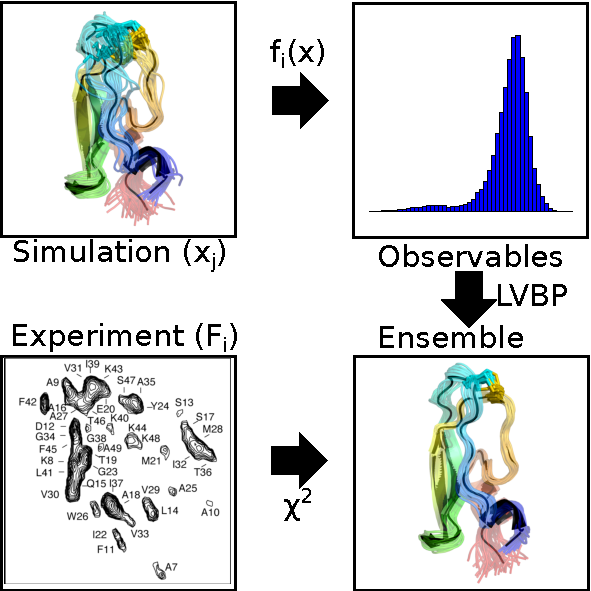
\includegraphics[width=18.0cm]{figures/info_graphic/info_graphic.pdf}

\caption{
General scheme for LVBP modelling.
}
\label{figure:LVBP}
\end{figure}

\subsection{Reweighting}

The next step in constructing an ensemble is to calculate the population of each conformation.  For convenience, we work with the $\log$ populations (i.e. free energies). Inspired by a previous method for restraining simulations \cite{chodera2012}, we reweight individual conformations by a biasing potential that is a linear combination of the predicted observables:

$$\Delta U(x;\alpha) = \sum_i^n \alpha_i f_i(x)$$

In $\Delta U(x;\alpha)$, the parameters $\alpha_i$ determine how strongly each experiment contributes to the biasing potential.  One way to think about $\alpha$ is via ``tilting'' the energy landscape along the order parameters $f_i(x)$.  Given the biasing potential, the population of each conformation can be calculated using exponential averaging (see Appx. S1):

$$\pi_j(\alpha) = \frac{1}{\sum_k \exp[-\Delta U(x_k;\alpha)]} \exp[-\Delta U(x_j;\alpha)]$$

It is informative to consider the case of a single observable $f(x)$.  Suppose the molecule of interest shows a normally distributed observable.  If we let $\alpha$ = 0, then the biasing potential is $0$ everywhere and our reweighted ensemble simply returns the results of the MD simulation (Fig. \ref{figure:Hist}b).  However, if we let $\alpha = -2$, conformations with large values of $f(x)$ are upweighted, while conformations with lower values of $f(x)$ are downweighted (Fig. \ref{figure:Hist}a).  Finally, if $\alpha = +2$, the ensemble shifts in the opposite direction (Fig. \ref{figure:Hist}c).  

\begin{figure}

\subfigure[]{
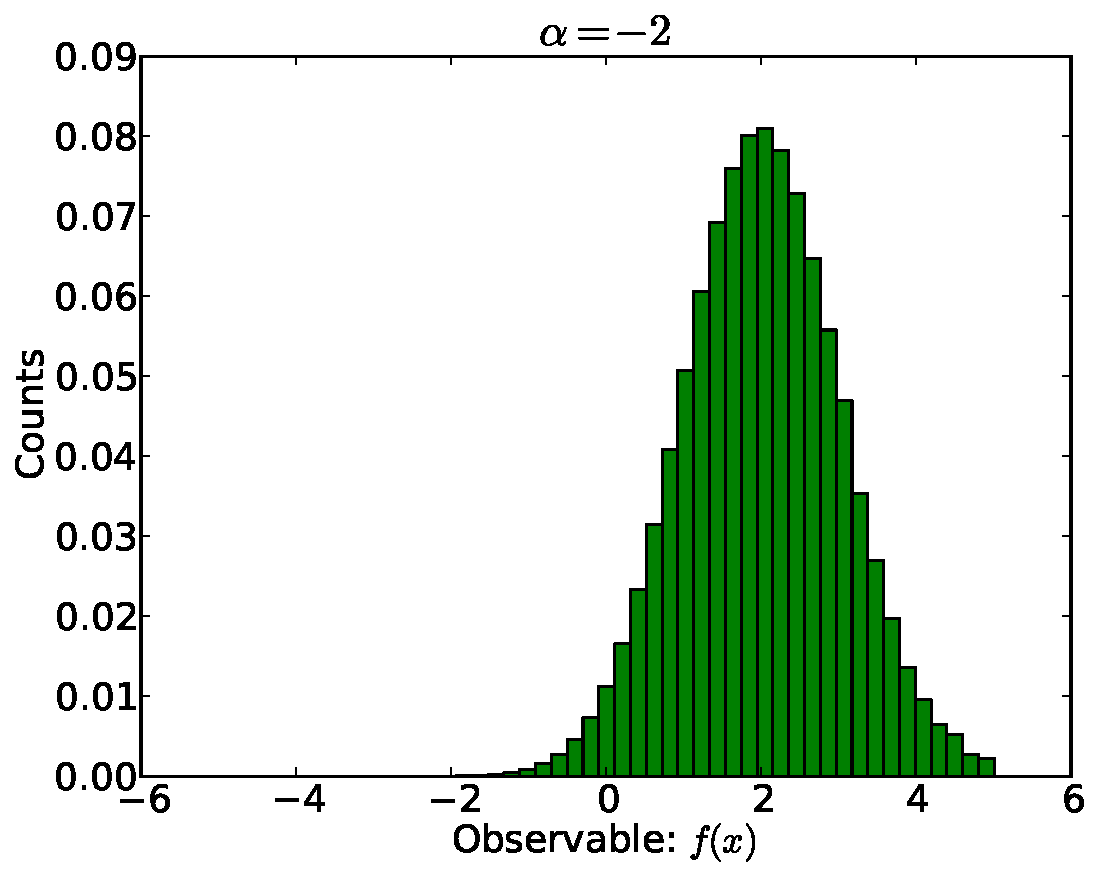
\includegraphics[width=5.0cm]{figures/model_hist-2.pdf}
}
\subfigure[]{
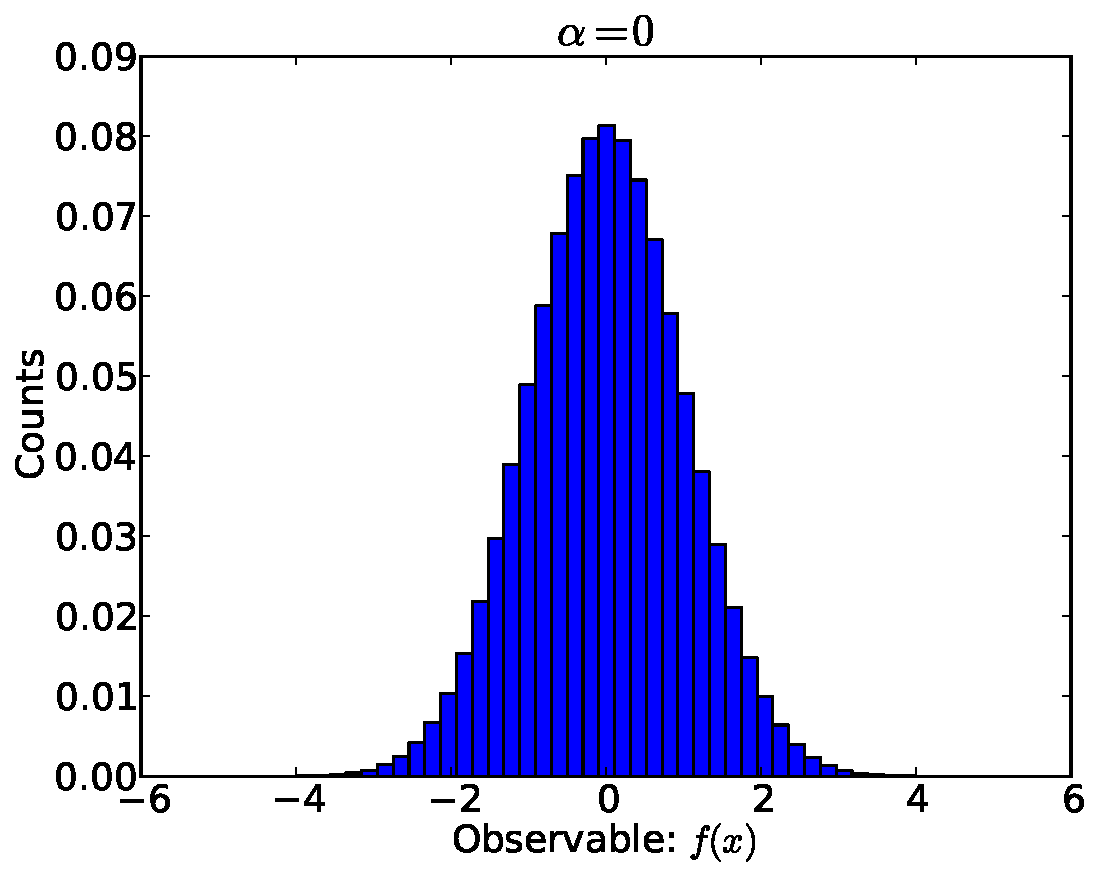
\includegraphics[width=5.0cm]{figures/model_hist0.pdf}
}
\subfigure[]{
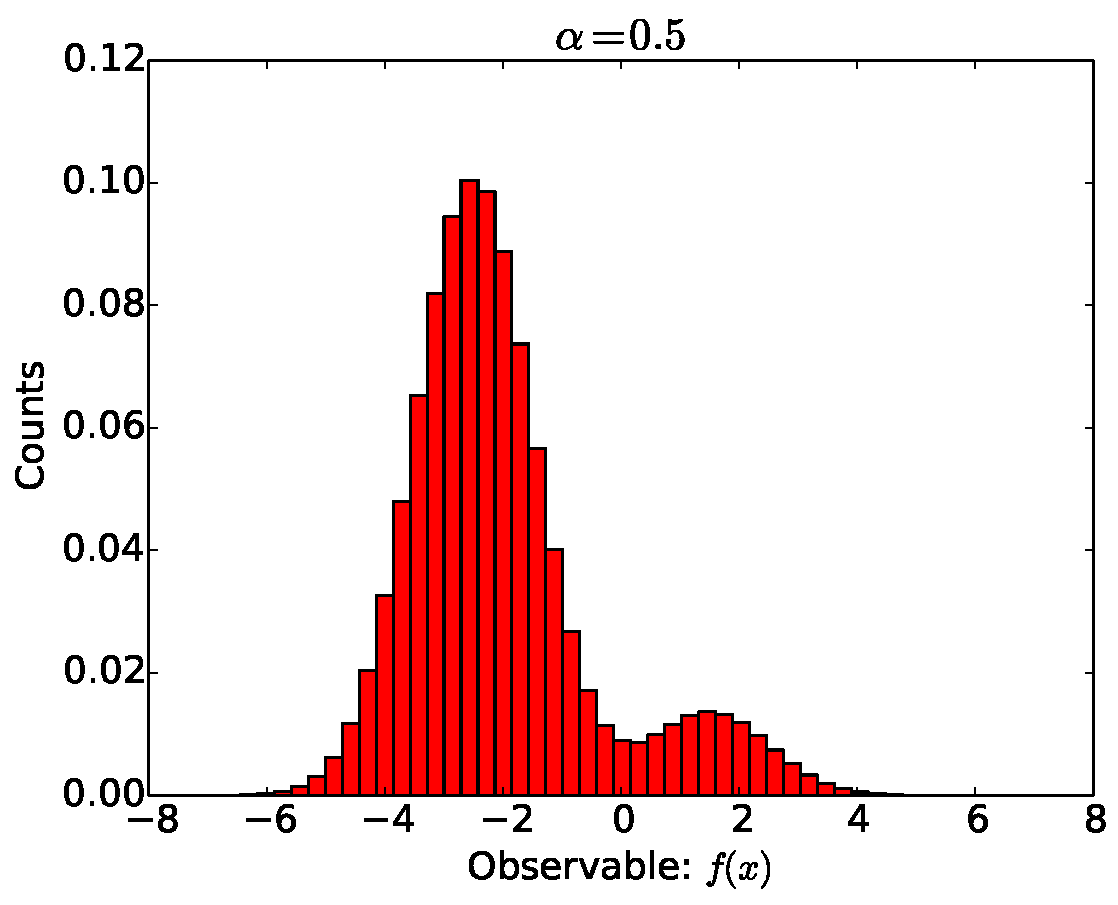
\includegraphics[width=5.0cm]{figures/model_hist2.pdf}
}
\caption{
Raw ($\alpha = 0$) and reweighted histograms of a one dimensional observable.
}
\label{figure:Hist}
\end{figure}

With the equilibrium populations, we can calculate the equilibrium expectations of an arbitrary observable $h(x)$:

$$\langle h(x)\rangle _\alpha = \sum_j h(x_j) \pi_j(\alpha)$$

In the above bracket notation, $\langle h(x)\rangle _\alpha$ is the ensemble average of $h(x)$ in an ensemble that is perturbed by a biasing potential $\Delta U(x;\alpha)$.  At this point, the determination of $\alpha$ has not yet been discussed.  The key idea, however, is that the $\alpha$ reweighted ensemble $\langle \rangle _\alpha$ should recapitulate the experimental measurements:

$$\langle f_i(x)\rangle _\alpha \approx F_i$$


\subsection{A likelihood framework}

We now derive a likelihood framework for determining the coefficients $\alpha$ used in the biasing potential.  Given adequate sampling and self-consistent experiments, there should exist some \emph{true} value of $\alpha$ whose ensemble matches the experimental data.  However, experimental uncertainty ($\sigma_i)$ prevents exact agreement between the measurements and the true ensemble.  For the models in the current work, we model $\sigma_i$ as the uncertainty associated with predicting chemical shifts and scalar couplings from structures; this dominant error is quantified by the RMS uncertainty estimated during the parameterization of chemical shift and scalar coupling models.  We use an independent normal approximation (see Appx. S2) to model the agreement between the $\alpha$ ensemble and the measurements:

$$P(F_i | \alpha) \sim N(\langle f_i(x)\rangle _\alpha, \sigma_i^2)$$

Using Bayes Theorem, we can calculate the likelihood of $\alpha$ given the measurements:

$$P(\alpha | F_1, ..., F_n) \propto P(F_1, ..., F_n | \alpha) P(\alpha)$$

Now we let $LL(\alpha)$ denote the log likelihood of $\alpha$ and simplify, dropping terms that are independent of $\alpha$:

$$LL(\alpha) = \log[ P(\alpha|F_1, ..., F_n)] = -\sum_i \frac{1}{2\sigma_i^2}(\langle f_i\rangle _\alpha - F_i)^2 + \log P(\alpha)$$

Note the simple form of the log likelihood.  The first term measures the $\chi^2$ agreement between the reweighted ensemble and measurements.  The second term is the log of the prior distribution on $\alpha$.  Although other priors are possible (see Appxs. S3, S4), we recommend a maximum entropy prior, which penalizes ensembles as they deviate from the raw simulation results:

$$\log P(\alpha) = \lambda \sum_j \pi_j(\alpha) \log \pi_j(\alpha)$$

With large values of $\lambda$, the maximum entropy prior favors the raw simulation results (i.e. uniform conformational populations): $\pi_i \approx \frac{1}{n}$.  The value of $\lambda$ can be chosen via cross-validation or other methods (see Appx. S5).  

\subsection{Bayesian Modeling of Structural Ensembles}

Because ensemble inference often presents many plausible solutions \cite{fisher2010, rieping2005}, we avoid statistical methods that return a single solution (e.g. maximum likelihood) .  We therefore use Markov chain Monte Carlo (MCMC), as implemented in PyMC \cite{patil2010pymc}, to sample the distribution of structural ensembles consistent with experiment.  The result is an ensemble of ensembles--a statistical ensemble of conformational ensembles.  Averaging all MCMC samples provides posterior mean  estimates of arbitrary structural features.  Similarly, examining the MCMC variances provides statistical uncertainties.  The shape of the posterior distribution indicates whether one or several models are consistent with the available data (Fig. S1).  A Bayesian bootstrapping procedure \cite{rubin1981} can also be used to model the statistical uncertainty of the MD simulations (see Appx. S6).

\section{Results}

\subsection{Conformational Propensities of Trialanine}

Short peptides provide crucial tests for evaluating and optimizing molecular dynamics forcefields \cite{Graf2007,beauchamp2012protein, Nerenberg2011, Best2008, Grdadolnik2011}.  Such peptides offer a window into the intrinsic conformational propensities of amino acids, free from the secondary structure bias found in statistical surveys of protein structures \cite{Jha2005}.  Here, we use LVBP to infer the conformational populations of trialanine from chemical shift and scalar coupling measurements \cite{Graf2007}.  

Trialanine was simulated (see Methods) in five different force fields; nine experimental measurements (six scalar couplings, three chemical shifts) probing the central ALA residue were used to construct an LVBP ensemble.  The five force fields show considerable variation in their agreement with experiment (Fig. \ref{figure:ALA3}a).  The amber96, amber99, charmm27, and oplsaa forcefields, for example, initially show significant deviation from the experimental measurements.  Upon reweighting, however, all five forcefields agree with experiment.  

\begin{figure}
\subfigure[]{
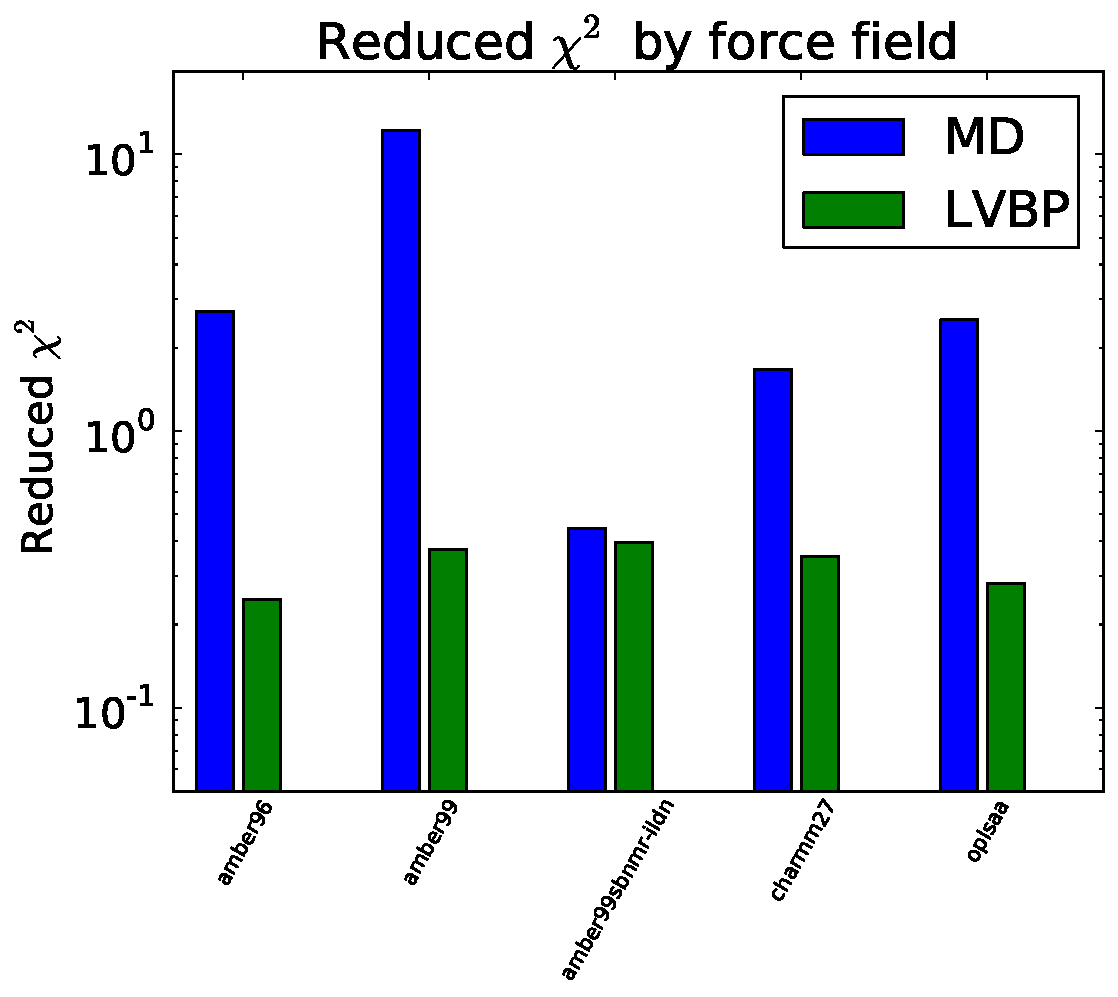
\includegraphics[width=7.5cm]{figures/ALA3_chi2.pdf}
}
\subfigure[]{
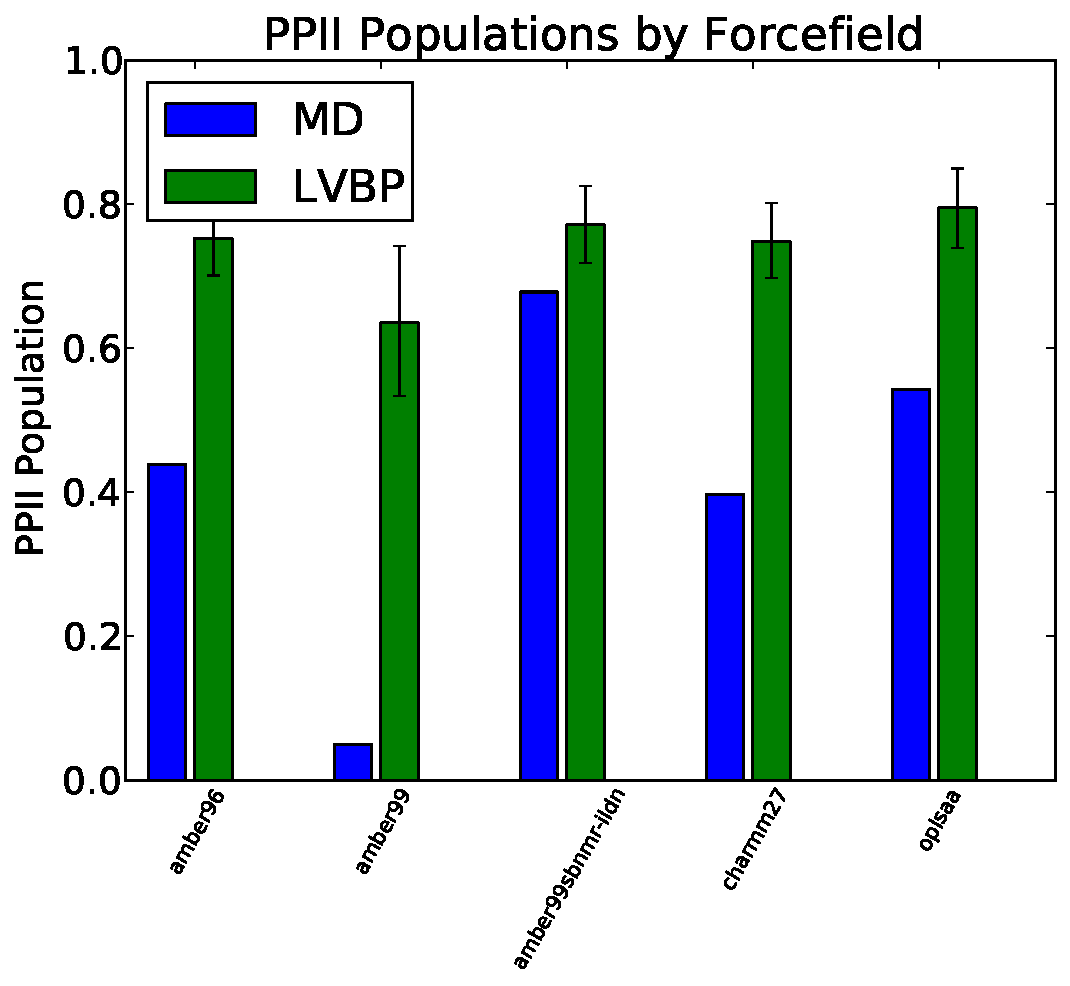
\includegraphics[width=7.5cm]{figures/state_0_by_forcefield.pdf}
}

\subfigure[]{
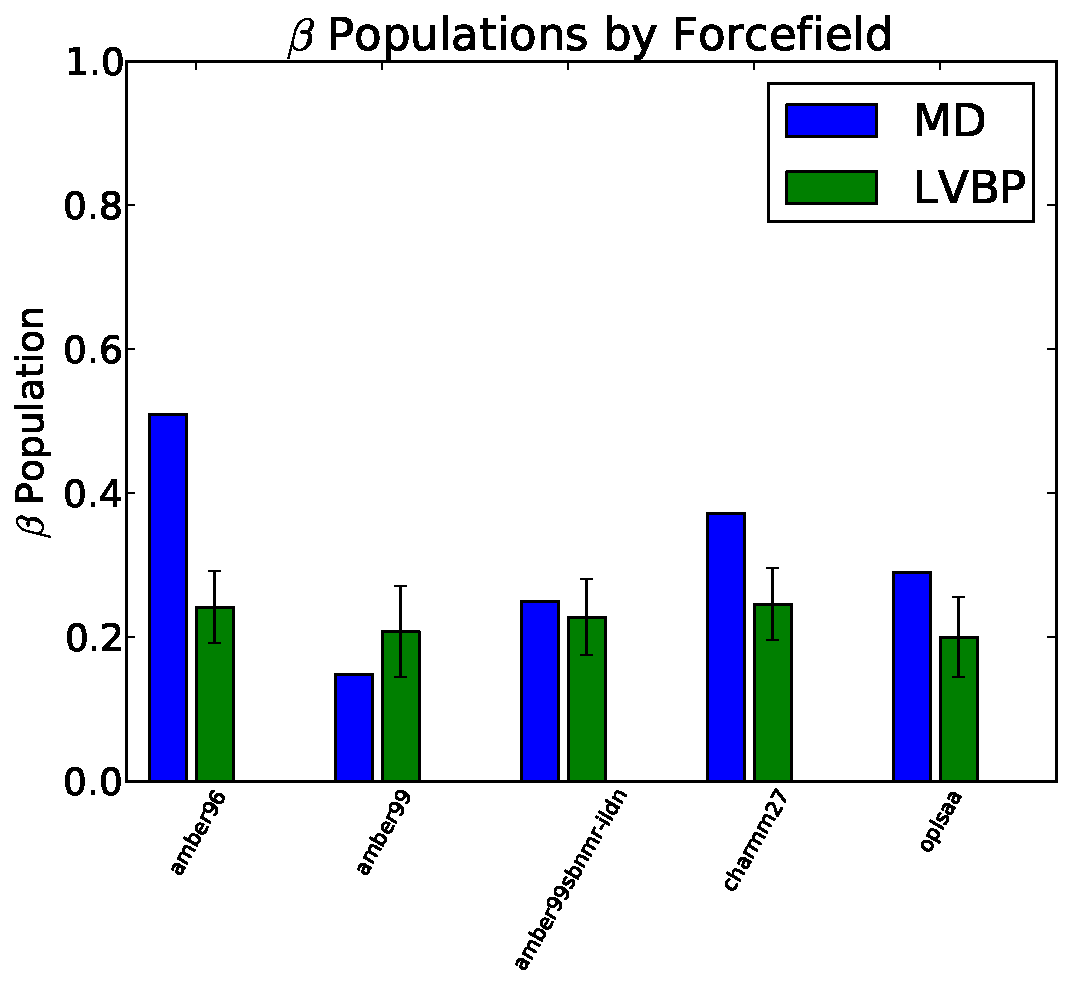
\includegraphics[width=7.5cm]{figures/state_1_by_forcefield.pdf}
}
\subfigure[]{
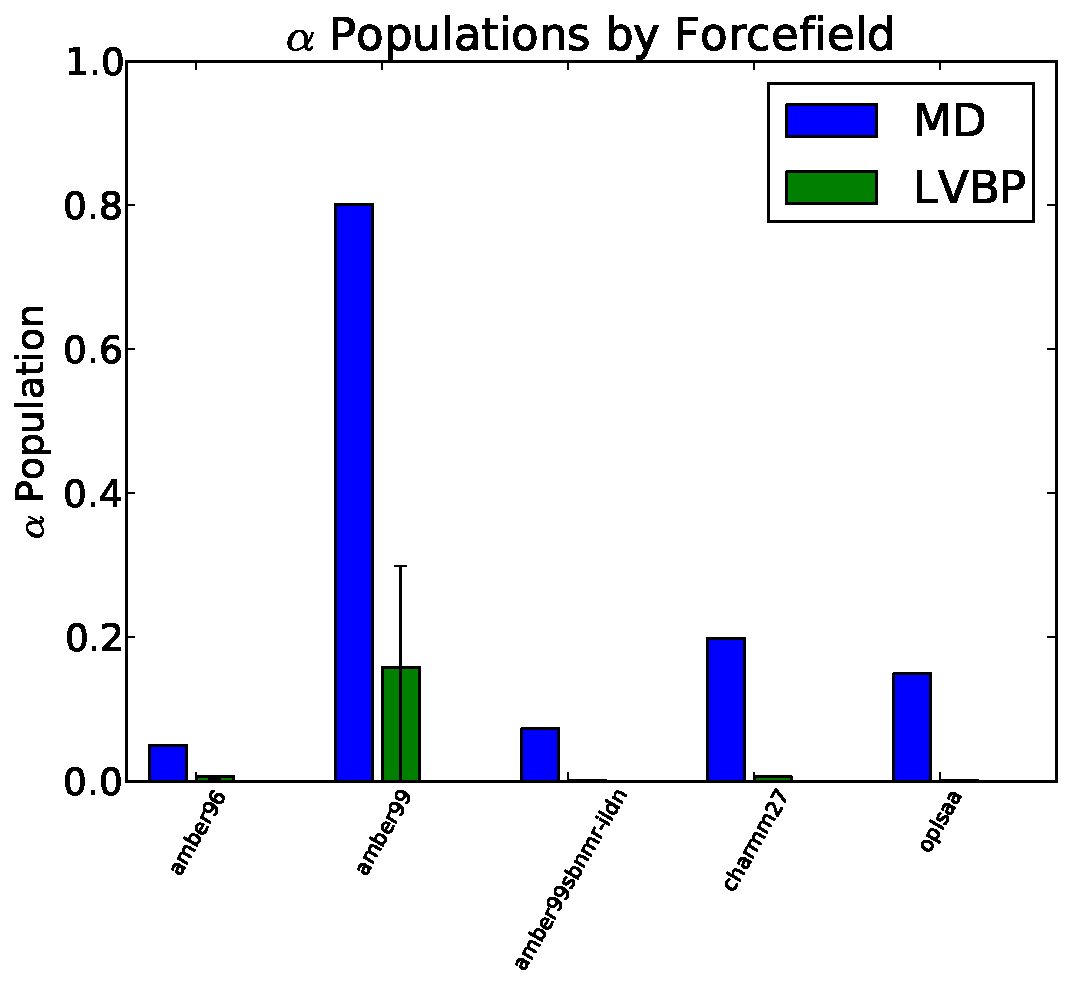
\includegraphics[width=7.5cm]{figures/state_2_by_forcefield.pdf}
}
\caption{
(a).  The reduced $\chi^2$ error for each raw and reweighted simulation.  The LVBP reduced $\chi^2$ is estimated as the mean reduced $\chi^2$ over all MCMC samples.  (b-d).  Raw and reweighted conformational propensities for each force field.  Note that amber99 shows larger uncertainties due to the extremely limited amount of $PP_{II}$ sampling in the amber99 forcefield.
}
\label{figure:ALA3}
\end{figure}


Previous experimental studies have shown that short alanine peptides prefer the polyproline type helix (PPII) in solution \cite{Grdadolnik2011, Graf2007, Avbelj2006}.  Most molecular dynamics forcefields, however, are known to underpopulate the PPII state \cite{Graf2007,beauchamp2012protein,Nerenberg2011, Best2008}.  Our trialanine simulations recapitulate this known deficiency (Fig. \ref{figure:ALA3} b-d; blue), with amber96 showing a strong $\beta$ bias and amber99 showing a strong $\alpha$ bias.  However, combining simulation and experiment leads to conformational ensembles that are robust to forcefield differences (Fig. \ref{figure:ALA3} b-d, green; Fig. S2).  Reweighting with limited experimental data is a powerful technique for correcting forcefield deficiencies.  


\section{Discussion}

\subsection{Structural (Ensemble?) Biology}

Why model structural ensembles, rather than just structures?  At least three compelling reasons favor ensembles.  First, biological molecules are multi-state machines; they fold, unfold, bind ligands, aggregate, and change conformation.  Biology is controlled by the relative populations of these states.  Structural ensembles capture aspects of these phenomena by encoding equilibrium populations.  A second argument for ensemble modelling is fidelity to experiment.  Most solution experiments measure ensemble average equilibrium properties--chemical shifts, scalar couplings, NOEs, SAXS, and FRET are reasonably well-described as equilibrium properties.  A truly quantitative connection to these measurements requires modelling the equilibrium ensemble.  Finally, recent advances in atomistic simulation \cite{hess2008, pronk2013gromacs, eastman2012openmm, eastman2010openmm}, special-purpose hardware \cite{Shaw2008}, and distributed computing analysis \cite{emma, msmb2} have enabled atomistic simulations to reach the 
millisecond 
timescale \cite{voelz2010, bowman2011atomistic, Shaw2010, Shaw2011}; the computational cost of ensemble modeling is quickly becoming manageable.

One might argue that structural ensembles are unnecessary because many proteins occupy a single state under physiological conditions.  For such proteins, it is probably safe to enforce single state behavior, as is done in current modelling approaches. However, we suggest that the number of states be \emph{inferred}--not \emph{assumed}.  

\subsection{Comparison to previous methods}

LVBP offers several key advantages over previous ensemble estimation techniques.  Most previous ensemble modeling efforts involve a protocol that involves three key ingredients: clustering, a $\chi^2$ objective function, and population inference on the clusters.  For example, this recipe describes the approach used in previous analyses of homopeptides \cite{graf2005}, the EROS inference technique \cite{rozycki2011saxs}, and the Bayesian Weighting formalism \cite{fisher2010}.  In our opinion, the primary disadvantage of these techniques is the need for a clustering step.  The clustering step can introduce two forms of error.  First, clustering can overly coarsen the system of interest.  For example, too few states could prevent the model from reproducing multiple experimental observables.  At the other extreme, too many states could lead to over-fitting and sensitivity to prior--this is because one needs to estimate a large number of populations.  This will lead to poor generalization performance--high errors 
when predicting experiments \emph{not} used to train the model.  

In contrast, LVBP avoids clustering by projecting simulations onto a basis defined by the predicted experimental observables.  The advantage of working in this basis are threefold.  

First, in LVBP, one estimates a single parameter ($\alpha_i$) for each experimental observable.  If the experiments is small, as is often the case, the inference problem has only a few parameters to estimate.  

Second, the predicted observables are a \emph{natural} basis for biophysical calculations.  This basis allows direct connection to experiment and often provides insight into the molecular interactions driving biophysical phenenoma.  For example, the projection onto observables could be used to rationally infer forcefield parameters, similar to ForceBalance method \cite{LeePing}.  

Third, suppose two conformations have the same predicted experimental observables.  In LVBP, these conformations will have the same population.  In clustering based methods, the populations of these conformations could vary simply due to random fluctuations.  

Finally, in the limit of exact measurements, LVBP gives the same answer as a previous \cite{chodera2012} maximum entropy approach (see Appx. SX).  

These reasons provide a theoretical basis supporting the LVBP method.  However, it is possible to evaluate the method \emph{quantitatively}.  One hallmark of a good statistical model is its predictive ability on set-aside test data \cite{friedman2001elements}.  We therefore fit BW models on the training data and evaluated on the set-aside test data.  For four out of five force fields, we find that the LVBP models outperform the raw MD models and the BW model with few (4) and many (144) states, respectively.  Our four state model consists of the $(\phi, \psi)$ based secondary structure assignments \cite{Jha2005} ($\alpha_r$, $\beta$, $PP_{II}$, and other).  Our 144 state model was constructed by dividing the ramachandran plot into square bins of $30\times30$ degrees.  Although the BW models outperform LVBP in one case, this case happens to be for the amber99sbnmr-ildn forcefield.  That forcefield was \emph{fit} to match NMR observables; the raw MD simulation has a reduced $\chi^2$ well below 1.  This suggests that all 
methods (raw MD, LVBP, and BW) are consistent with experiment.  

\begin{math}
\begin{tabular}{lrrrrr}
\toprule
{} &   amber96 &   amber99 &  amber99sbnmr-ildn &  charmm27 &    oplsaa \\
\midrule
maxent &  0.776853 &  0.980453 &           1.008226 &  0.931457 &  1.090944 \\
MVN    &  0.838097 &  1.033197 &           0.942220 &  0.939043 &  1.067730 \\
BW     &  0.973795 &  1.472812 &           0.735458 &  1.061796 &  1.990149 \\
BW12   &  1.507146 &  3.011690 &           0.469157 &  1.090342 &  2.341762 \\
MD     &  1.508180 &  3.199790 &           0.644300 &  1.161881 &  2.310684 \\
\bottomrule
\end{tabular}
\end{math}

\section{Future Work}

The LVBP method can be extended in several ways.  We have already worked out some of these extensions.  In App. SX, we derive an approximate correction for working with dependent data.  Another obvious extension is the use of non-Normal error models.  These models can be directly inserted into the current framework by replacing the $\chi^2$ term in the likelihood with some other loss function.  

More sophisticated models could separately treat the uncertainties associated with predicting observables and the uncertainties of conformations.  This would replace the regularization and Bayesian Bootstrapping (App. SX) approaches1 used herein.  In such a model, it is likely that both the prediction and conformational uncertainties are non-normal; future work will be useful for exploring such models.  As a concrete example, one possible error model might involve taking the $\max$ of the prediction uncertainty and the conformational uncertainty for a given reweighted observable.  


\section{Conclusion}

Bayesian inference of conformational ensembles allows the simultaneous characterization of structural and equilibrium properties.  Limited experimental data can be used to supplement equilibrium simulations, leading to predictions that are robust to forcefield error and consistent with available measurements.  Our equilibrium ensemble of BPTI suggests coupled motion in the trypsin specificity loop and the C14-C38 disulfide bridge.  Falsifying or refining the present model offers a key challenge for understanding the conformational fluctuations in BPTI.

\section{Acknowledgements}

We thank John Chodera, TJ Lane, Frank Cochran, Pehr Harbury, Xuesong Shi, and Dan Herschlag for helpful discussions.  We thank DE Shaw research for providing the millisecond simulation of BPTI.  

\section{Methods}

\subsection{Methods: Trialanine}

Trialanine was simulated in the amber96\cite{kollman1996}, amber99\cite{wang2000}, amber99sbnmr-ildn\cite{li2010}, charmm27\cite{mackerell2004extending,bjelkmar2010implementation}, and oplsaa\cite{kaminski2001evaluation} force fields, as previously reported \cite{beauchamp2012protein}.  Simulations were performed using Gromacs 4.5 \cite{hess2008} and run at constant temperature (300 K) and pressure (1.01 atm).  Each simulation was at least 225 ns long.  Conformations were stored every 5 ps.  Chemical shifts (H, HA, CA, CB) for each frame were calculated using the average prediction of ShiftX2\cite{han2011shiftx2}, SPARTA+ \cite{Shen2010}, and PPM\cite{li2012ppm}; uncertainties were estimated as the mean uncertainty reported by SPARTA+. J couplings were calculated using the following Karplus relations: $^3J(H^N C')$ \cite{Schmidt1999}, $^3J(H^N H^\alpha)$ \cite{vogeli2007limits}, $^2J(N C^\alpha)$ \cite{Graf2007}, $^3J(H^\alpha C')$ \cite{Schmidt1999}, $^1J(N C^\alpha)$ \cite{Graf2007}, $^3J(H^N C^\beta)$ \
cite{vogeli2007limits}.  J coupling uncertainties were approximated as the RMS errors reported when fitting the Karplus coefficients.  


\bibliography{lvbp}


\end{document}